\documentclass[11pt]{article}

\usepackage[margin=1in]{geometry}
\usepackage[T1]{fontenc}
\usepackage[utf8]{inputenc}
\usepackage{lmodern}
\usepackage{microtype}
\usepackage{amsmath}
\usepackage{booktabs}
\usepackage{threeparttable}
\usepackage{siunitx}
\usepackage{pgfplots}
\pgfplotsset{compat=1.17}
\usepackage[authoryear,round]{natbib}
\usepackage[hidelinks]{hyperref}
\usepackage{setspace}
\setstretch{1.1}

\sisetup{detect-all, group-minimum-digits=4}
\newcommand{\pp}{\,pp}

\title{The Invention, Not the Inventor:\\Patent Renewal by Emerging-Market Firms}
\author{Samuel Edet\thanks{[Affiliation]. Email: samueledet@aims.ac.za. [Disclaimer and acknowledgements.]}}
\date{Draft, October 2026}

\begin{document}
\maketitle

\begin{abstract}
\noindent Patents owned by firms in emerging markets lapse sooner than those of foreign owners in the same
office, which is often read as a sign that the inventions are worth less to their owners or that the owners cannot
afford to use them. Using renewal records for 2.6 million firm and university patents at the patent offices of
China, Korea, Brazil, the United States, Japan, Germany and the United Kingdom, I show that most of this gap is a
timing artefact: domestic patents in China and Korea are granted about two years earlier than foreign ones, and
renewal fees start at grant. Measured from grant and compared at equal observable quality, emerging-market firms
of every size keep their patents at least as long as firms in rich economies. Evidence from the same inventions
patented at home and abroad, credit shocks, fee changes and two structural renewal models, including
patent-level values estimated without reference to owner type, points the same way. Two differences remain:
small emerging-market firms' patents gain more from being sold, and Chinese university patents are worth well
under half as much as comparable foreign ones.

\medskip
\noindent\textbf{Keywords:} patent renewal, patent value, emerging markets, innovation, intellectual property\\
\noindent\textbf{JEL:} O34, O31, O32, L26
\end{abstract}

\section{Introduction}

Emerging economies now account for a large share of the world's patenting: China's patent office alone received
49\% of the 3.7 million patent applications filed worldwide in 2024, up from 35\% in 2014 \citep{WIPO2025}. Yet
their patents are widely thought to be worth less. Renewal decisions offer a direct test. Owners pay a fee every year to keep a patent in force and stop paying
once it is no longer worth the fee, so the age at which patents lapse reveals what they are worth to their owners
\citep{PakesSchankerman1984,Pakes1986,SchankermanPakes1986}. By this measure the gap looks large. In the Chinese
patent office, patents filed in 2000--2005 by domestic firms were 13 percentage points less likely than those of
foreign owners to be alive eight years after grant.

Two very different stories fit such a gap. In the first, the \emph{invention} is the problem: emerging-market
patents protect weaker technology, and owners rationally drop them sooner. In the second, the \emph{inventor} is
the problem: owners lack the finance, production capacity or market access to turn valuable inventions into
returns, so good patents lapse for want of an owner able to use them. The policy response differ. The first calls
for investment in research capability and links to frontier technology; the second for credit, fee relief or
markets in which patents can find better owners.

This paper separates the two using the legal-event records in PATSTAT, which track renewals and lapses at the
offices that report them. I first establish which offices do: of the large emerging economies, only China, Korea,
Russia, Taiwan and the Czech Republic record lapses consistently and have enough domestic firm
patents.\footnote{India, Mexico, South Africa and most of Latin America, Africa and South-East Asia report no lapses
to PATSTAT; Brazil and Hungary report them but have too few domestic firm patents (Appendix~\ref{app:data}).}
I compare these against five advanced economies (the United States, Japan, Germany, the United Kingdom, and France) using a dataset of approximately three million granted patents held by firms and universities, complemented with the historical renewal-fee schedules compiled from official patent-office sources. The design compares domestic and foreign owners in the same office (exposed to the same fees, law and
enforcement), and asks whether the domestic shortfall is larger in emerging-market offices. The paper makes four
points.

First, the raw shortfall reflects what is patented. Domestic patents in emerging-market offices are cited far less
than foreign ones, and once citations, technology field and owner type are held fixed, the extra domestic shortfall in
emerging-market offices disappears: larger emerging-market firms keep their patents longer than comparable firms in
the advanced economies, and small firms about as long, within a few points either way depending on the quality
controls and on which advanced economies form the benchmark (Section~\ref{sec:survival}). The result holds in China and Korea, but imprecise in the Czech Republic, and
fails for small firms in Russia and, more weakly, in Taiwan.

Second, there is no sign that emerging-market owners are held back by finance or by the cost of renewal
(Section~\ref{sec:constraints}). Small firms everywhere keep the home patent of an invention longer than its
foreign patents, and more so in the emerging economies, the opposite of what owners unable to use their home patents
would do. Credit crunches do not raise small domestic firms' lapses in the emerging economies. And small firms respond only weakly to large fee cuts.

Third, structural renewal models turn these decisions into money (Section~\ref{sec:values}). Valuing each patent from its own renewal history,
without reference to its owner, the home premium (the value of domestic relative to foreign owners' patents in the
same office) is as large in the emerging-market offices as in the advanced ones for all owners together and for
mid-sized and large firms. For small firms it is smaller against the advanced-economy pool, which Japan dominates;
office by office, small firms' premium in China and Korea is as large as in the United States and Germany. The results
hold when every eligible owner is assumed to pay discounted fees provided by Chinese and Korean patent office.

Fourth, two differences remain. Patents sold by small emerging-market firms survive much longer afterwards than
patents sold by small firms in the advanced economies, which suggests that owner capacity matters at the margin and that markets for
technology move patents to better owners. And university patents in China are the one robust weak spot: they lapse
sooner and are worth well under half as much as foreign universities' patents at equal quality. Here the owner
matters too: once sold, Chinese university patents survive 45 points longer, while a sale does not raise the survival of
university patents in the advanced economies. This implies that Chinese universities hold patents that firms find worth keeping but
that they do not use themselves.

I close by pricing the policy levers on a common scale (Section~\ref{sec:stake}). Had every eligible owner taken up
China's and Korea's fee discounts, the returns from a cohort of small firms' patents would barely have changed. Had patents held by small firms generated the same returns as those realized by their buyers, aggregate returns would have increased by up to \$250 million per cohort in China and \$80 million in Korea --- this rises to \$1.1 billion and \$143 million for all domestic owners, universities included, in China and Korea respectively. Similarly, if Chinese universities' patents had generated returns comparable to those of foreign universities operating in China, the gains would have ranged from \$170 million to \$310 million. These are private returns, not welfare, but the ordering is clear: the gains lie in markets for
technology and in what universities patent, not in cheaper renewal.

The paper contributes to three literatures. The first estimates the value of patent rights from renewal decisions
\citep{PakesSchankerman1984,Pakes1986,SchankermanPakes1986,Lanjouw1998,Bessen2008}; I extend it to emerging-market
offices, with fee histories for ten offices over 25 years. The second studies indicators of patent value
\citep{HarhoffSchererVopel2003,HallJaffeTrajtenberg2005,KoganEtAl2017}; I value each patent from its own renewal
path rather than from its owner's characteristics. The third asks whether Chinese and other emerging-market patenting
is of low quality \citep{HuJefferson2009,LiegsalzWagner2013,DangMotohashi2015}; the answer here is that, for firms,
lower survival reflects the technology, not the owners' ability to use their patents. The sale premium connects to
work on markets for patents \citep{Serrano2010,GalassoSchankermanSerrano2013}.

Section~\ref{sec:data} describes the data and design. Section~\ref{sec:survival} compares survival at equal
quality, Section~\ref{sec:constraints} tests for owner constraints, Section~\ref{sec:values} turns renewal decisions
into money, and Section~\ref{sec:stake} compares policy levers. Section~\ref{sec:conclusion} concludes.

\section{Data and measurement}\label{sec:data}

\paragraph{Patents and lapses.} The data are PATSTAT Global (Autumn 2025 edition). The sample is granted invention
patents filed in 2000--2005 at the offices of China, Korea and Brazil (the emerging-market offices) and the
United States, Japan, Germany and the United Kingdom, all of which record lapses in the INPADOC legal-event table.
These cohorts can be followed for close to twenty years. A patent lapses at its first cessation event before
19.5~years from filing; later cessations are expiry at full term.

\paragraph{Owners.} Owner country is the first applicant's country, imputed from the patent family and the office
of first filing where it is missing (mainly in China and Japan). Owners are grouped by sector and by size, measured
as the number of distinct patent families their harmonised applicant identity filed in 2000--2020: firms with
1--9, 10--99, 100--999 and 1{,}000 or more families, and universities and public research organisations.
Individual inventors are excluded: their patents behave differently, and in China they were the main target of
local filing subsidies in this period. ``Small firms'' are firms with 1--9 families. The main sample has
2.6~million patents with a grant lag of up to ten years.

\paragraph{Quality.} Observable quality is measured by forward citations to the patent family (logged), citations
that block later claims (X and Y categories), citations received by age four, family size and the WIPO technology
field (35 fields). Claims are recorded only for US publications.

\paragraph{Design.} The basic comparison is between domestic and foreign owners in the same office, which holds
fees, law and enforcement fixed. The emerging-market question is whether that domestic gap is larger in the
emerging-market offices than in the rich-economy ones: a difference in differences, estimated as a linear
probability model with office $\times$ filing-year and office $\times$ field fixed effects, office-specific
citation slopes and office $\times$ owner-group effects. Standard errors are clustered by owner.

\paragraph{Fees.} Renewal fee schedules for the seven offices were compiled from official sources by year of life
and period. For the structural models, fees are deflated to 2024 prices with each country's consumer price index
for the year paid and converted at 2024 purchasing-power parities \citep[World Development Indicators;][]{WDI};
fees due after 2024 are held fixed in 2024 prices.

\section{The timing artefact}\label{sec:timing}

Renewal fees are due from grant, not from filing. If two otherwise identical patents are filed on the same day and
one is granted two years earlier, by ten years from filing its owner has faced two more renewal decisions, and it
is more likely to have lapsed for that reason alone. Comparisons of survival from filing therefore mix value with
exposure whenever grant speeds differ between the groups being compared.

They differ sharply between domestic and foreign owners in China and Korea. For small owners, the median grant lag
is 3.5~years for domestic and 5.5~years for foreign patents in China, and 2.4 against 5.0~years in Korea; many
foreign applications enter through the PCT national phase, which adds time before examination starts. In the
rich-economy offices the domestic--foreign difference is about one year or less.

Table~\ref{tab:timing} and Figure~\ref{fig:timing} show the consequence. Measured as survival to ten years from
filing, with citation controls, small domestic firms in the emerging-market offices appear 8.4~points behind their
rich-economy counterparts, and universities 30~points behind. Adding X/Y citations or citations by age four changes
these figures by less than one point. Adding the grant lag closes most of the gap, and measuring survival from grant
reverses it for firms: by eight years after grant, emerging-market firms of every size are \emph{ahead} of
rich-economy firms relative to foreign owners in the same office. Only the university gap survives, at a third of
its original size.

\begin{table}[ht]
\centering
\begin{threeparttable}
\caption{The emerging-market gap, measured from filing and from grant}\label{tab:timing}
\small
% Source: em-patent-value notes sections 4 and 9 (09_heterogeneity.py, 16_rich_quality.py, 16c_survival_from_grant.py)
\begin{tabular}{lS[table-format=-2.1]S[table-format=-2.1]S[table-format=-2.1]}
\toprule
 & \multicolumn{2}{c}{Alive 10 years from filing} & {Alive 8 years} \\
\cmidrule(lr){2-3}
Owner group & {Citations} & {+ grant lag} & {from grant} \\
\midrule
Firms, 1--9 families     & -8.4  & 0.3   & 3.5 \\
Firms, 10--99            & -3.6  & {}    & 9.4 \\
Firms, 100--999          & -0.3  & 5.8   & 11.6 \\
Firms, 1{,}000+          & -2.4  & {}    & 6.2 \\
Universities             & -29.8 & -9.7  & -11.8 \\
\bottomrule
\end{tabular}
\begin{tablenotes}\footnotesize
\item Notes: Extra domestic--foreign gap in survival in the emerging-market offices (China, Korea, Brazil) relative to
the rich-economy offices, in percentage points. Linear probability models with office $\times$ year, office $\times$
field and office $\times$ owner-group fixed effects and office-specific citation slopes; owner groups estimated
jointly in the full sample. Standard errors (clustered by owner) are 0.5--3.5 points; see Appendix. Blank: not
estimated in that specification.
\end{tablenotes}
\end{threeparttable}
\end{table}

\begin{figure}[ht]
\centering
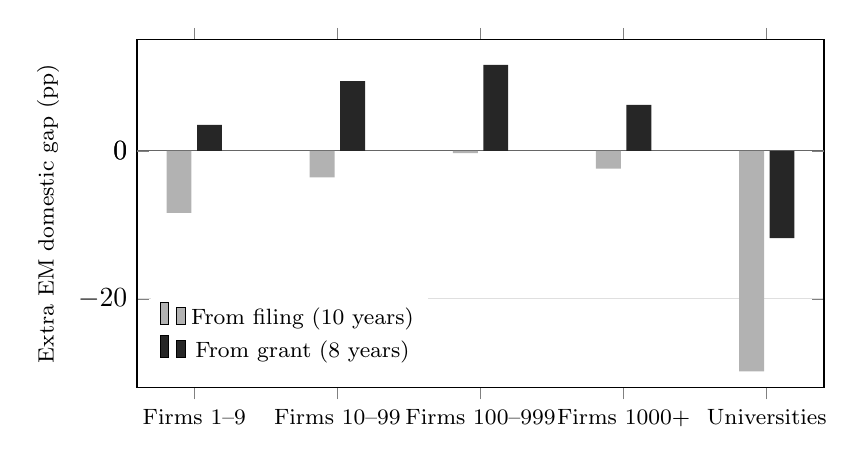
\begin{tikzpicture}
\begin{axis}[
  ybar, bar width=9pt, width=0.85\textwidth, height=6cm,
  symbolic x coords={Firms 1--9, Firms 10--99, Firms 100--999, Firms 1000+, Universities},
  xtick=data, x tick label style={font=\footnotesize, align=center},
  ylabel={Extra EM domestic gap (pp)}, ylabel style={font=\footnotesize},
  ymin=-32, ymax=15, ymajorgrids, grid style={gray!25},
  legend style={font=\footnotesize, at={(0.02,0.04)}, anchor=south west, draw=none},
  extra y ticks={0}, extra y tick style={grid=major, grid style={black!60}},
]
\addplot[fill=gray!60, draw=none] coordinates
  {(Firms 1--9,-8.4) (Firms 10--99,-3.6) (Firms 100--999,-0.3) (Firms 1000+,-2.4) (Universities,-29.8)};
\addplot[fill=black!85, draw=none] coordinates
  {(Firms 1--9,3.5) (Firms 10--99,9.4) (Firms 100--999,11.6) (Firms 1000+,6.2) (Universities,-11.8)};
\legend{From filing (10 years), From grant (8 years)}
\end{axis}
\end{tikzpicture}
\caption{Measured from grant, the emerging-market gap disappears for firms. Same estimates as
Table~\ref{tab:timing}.}\label{fig:timing}
\end{figure}

The lesson is general. Grant speeds differ across offices, owner nationalities, entry routes and periods, so any
comparison of patent survival or renewal-based value should start the clock at grant, or at the first renewal fee.

\section{Emerging-market firms at equal quality}\label{sec:survival}

\paragraph{Main estimates.} Table~\ref{tab:survival} reports the extra domestic gap in emerging-market offices,
measured as survival to eight years after grant. Without quality controls it is $-10.1$ (1.5) points: domestic
firms' patents in emerging-market offices are much less cited than foreign ones. With citation slopes, field and
owner-group effects it becomes $+4.3$ (1.5). The estimate is the same for the original set of offices
(China, Korea and the four largest advanced economies) and close to zero, $-0.5$ (1.9), when Korea and Taiwan, the
two high-income members of the emerging-market group, are left out. Richer quality controls (blocking citations, citations
by age four and office-specific slopes in the grant lag) lower the estimates for every firm size by 2--3 points
(Appendix Table~
ef{tab:rich}). Small emerging-market firms then come out 1.6 (0.6) points behind, and 3.0 (0.7)
with family size, which itself partly reflects owners' capacity to file abroad; larger firms remain 4--9 points
ahead. Small firms thus keep their patents about as long as small firms in the advanced economies, within a few
points either way, and larger firms longer.

\begin{table}[t]
\centering
\begin{threeparttable}
\caption{Extra domestic--foreign survival gap in emerging-market offices (percentage points)}\label{tab:survival}
\small
% Source: em-patent-value output/ext_overall.csv, ext_gradient.csv (23_extended_offices.py)
\begin{tabular}{lccc}
\toprule
 & All ten offices & Original six & Without Korea, Taiwan \\
 & (1) & (2) & (3) \\
\midrule
\multicolumn{4}{l}{\emph{A. All firms and universities}} \\
Alive 10 years from filing, raw            & $-18.4$ (1.6) & $-19.9$ (1.8) & $-25.8$ (2.1) \\
Alive 10 years from filing, quality controls & $-5.1$ (1.4) & $-6.2$ (1.5) & $-9.0$ (1.9) \\
Alive 8 years from grant, raw              & $-10.1$ (1.5) & $-11.5$ (1.7) & $-18.5$ (2.0) \\
Alive 8 years from grant, quality controls & \textbf{4.3} (1.5) & \textbf{4.3} (1.5) & $-0.5$ (1.9) \\
\addlinespace
\multicolumn{4}{l}{\emph{B. By owner group, alive 8 years from grant, quality controls}} \\
Firms, 1--9 families     & 1.7 (0.5)    & 3.4 (0.6)    & 2.6 (0.6) \\
Firms, 10--99            & 8.2 (0.9)    & 9.8 (1.0)    & 7.8 (1.2) \\
Firms, 100--999          & 9.3 (1.7)    & 12.3 (2.0)   & 10.1 (2.8) \\
Firms, 1{,}000+          & 9.3 (3.4)    & 6.6 (3.5)    & 4.8 (6.4) \\
Universities             & $-5.7$ (3.6) & $-11.5$ (3.1) & $-16.3$ (3.0) \\
\addlinespace
Patents                  & 2{,}961{,}829 & 2{,}615{,}050 & 2{,}439{,}754 \\
\bottomrule
\end{tabular}
\begin{tablenotes}\footnotesize
\item \emph{Notes:} Coefficient $\delta$ of equation~\eqref{eq:did}; standard errors clustered by owner in
parentheses. Raw: office $\times$ filing-year effects only. Quality controls: office-specific citation slopes, office
$\times$ field and (panel A) office $\times$ owner-group effects. Column (1): China, Korea, Russia, Taiwan and the Czech
Republic against the United States, Japan, Germany, the United Kingdom and France. Column (2): China and Korea against
the United States, Japan, Germany and the United Kingdom. Column (3): column (1) without Korea and Taiwan.
\end{tablenotes}
\end{threeparttable}
\end{table}

\paragraph{By country.} Figure~\ref{fig:country} compares each emerging-market office with the five advanced-economy
offices, by owner group. Chinese and Korean firms of every size are ahead: small firms by 4.0 (0.6) and 1.7 (1.1)
points, larger firms by 8--12 points. Czech firms are ahead by similar amounts, though with wide intervals. Russia is
the exception: small Russian firms are 5.9 (1.5) points behind, and Russian universities 11.9 (4.7). Small Taiwanese
firms are 3.8 (1.5) points behind, while large Taiwanese firms and universities are well ahead. Even the Russian and
Taiwanese shortfalls sit inside the range of domestic--foreign gaps among small firms in the advanced-economy
offices, from about zero in the United Kingdom to 18 points in Japan (Appendix Table~\ref{tab:within}).

\begin{figure}[t]
\centering
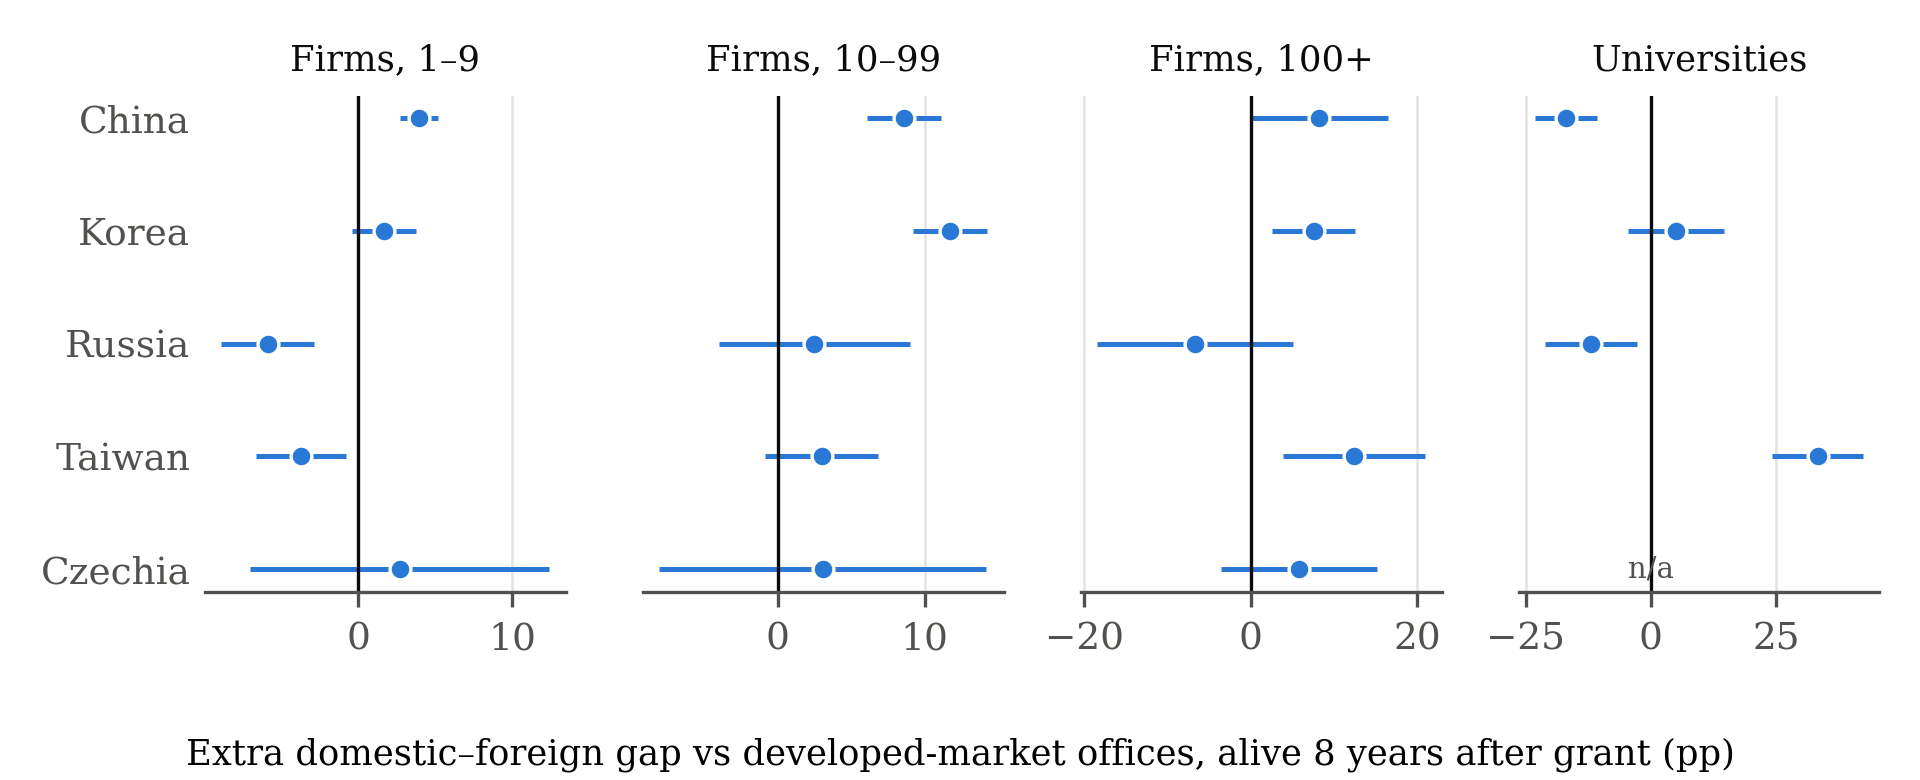
\includegraphics[width=0.9\textwidth]{figures/fig3_by_country.png}
\caption{Each emerging-market office against the advanced-economy offices}\label{fig:country}
\figurenotes{Coefficient $\delta$ of equation~\eqref{eq:did} estimated on one emerging-market office and the five
advanced-economy offices, separately for each owner group, with 95\% confidence intervals (standard errors clustered
by owner). Outcome: alive eight years after grant. The Czech Republic has too few domestic university patents (95).}
\end{figure}

\paragraph{Same invention, home and abroad.} Inventions patented both at home and in another study office hold the
technology fixed. With patent-family fixed effects, I compare how much longer small firms keep the home patent than
the same invention's foreign patents, relative to larger firms from the same country. If small emerging-market firms
found their home patents hard to use, they would drop them first. They do the opposite: small firms keep the home
patent relatively longer in China, by 10.2 (3.8) points, and Korea, by 9.9 (2.0), as in Japan (14.9), France (6.6)
and the United States (4.4); in Taiwan the difference is close to zero and in Russia it is imprecise (Appendix
Table~
ef{tab:same}). Small owners everywhere economise on
the expensive foreign patent first.

\paragraph{Credit shocks.} If finance were binding, credit crunches should raise small domestic firms' lapses. In a
patent-year panel with country-specific shock years (banking crises and documented credit crunches;
\citealp{LaevenValencia2018}), the interaction of shock, small owner and domestic owner is 0.37 points per year (0.75)
in the emerging-market offices and 0.23 (0.52) in the advanced-economy ones (Appendix Table~
ef{tab:credit}). Office $\times$ year effects
absorb fee changes and recording practices.

\paragraph{Fees.} Fee changes test cash constraints at renewal time directly. China's 85\% fee reduction for small
owners, whose window was extended from three to six fee-years in 2016 and to ten in 2018, lowers small firms' lapse
rate only slightly: an implied elasticity of 0.07 (intent to treat, since take-up is not observed). Small US firms
respond to stage-specific maintenance-fee changes with an elasticity of about 0.18. Small emerging-market firms are
not more fee-sensitive than small US firms.

\paragraph{Sales.} One result points to owner capacity at the margin. In a landmark design (patents alive and not
yet sold at ages 4--8, sold in the next year or not, outcome alive five years later, with citations counted only up
to the landmark age), a sale raises survival by 4.7 (0.7) points on average, by a further 8.3 (1.0) for small
emerging-market firms and by only 0.8 (1.0) for small advanced-economy firms
(Appendix Table~\ref{tab:credit}, panel B). Buyers select good patents everywhere, so the level of the premium is not causal;
the extra premium for small emerging-market sellers is the informative part. In China it is largest for sales to
other firms; in Russia there is none. Taiwan and the Czech Republic record no ownership transfers.

\section{What the patents are worth}\label{sec:values}

Survival is a coarse measure: it ignores how much fees differ between offices and over a patent's life. Renewal
models turn each patent's fee path and lapse decision into money. Fees come from official schedules for each of the
ten offices by year of life and period, deflated to 2024 prices with each country's consumer price index and
converted at 2024 purchasing-power parities \citep{WDI}.

\paragraph{Two models.} In the deterministic model \citep{SchankermanPakes1986}, a patent earns $r_0 d^t$ in year $t$
after grant, with $\ln r_0 \sim N(\alpha_g + \gamma \ln(1+c), \sigma)$ for owner group $g$ (domestic or foreign
$\times$ firm size or university). With returns falling and fees rising, the owner renews while returns over the
period a fee covers exceed the fee. In this model the rate of decline $1-d$ is not identified, so I also estimate the
learning model of \citet{Pakes1986}, in which log returns follow a random walk whose shocks shrink as owners learn,
and owners may keep a patent worth less than its fee for the option of later renewals. Where fees rise steeply every
year the decay rate is identified: 0.851 in Germany and 0.840 in the United Kingdom, close to the 0.85 commonly
assumed. I fix $d = 0.85$ everywhere. Appendix~\ref{app:models} gives the details.

\paragraph{The home premium is no smaller in most emerging markets.} Domestic owners value their patents more than
foreign owners in the same office, as they should: the home market is where they sell. The question is whether that
home premium is smaller in emerging markets. Figure~\ref{fig:values} shows that for China, Korea and the Czech
Republic it is not. At equal citations, the median small domestic firm's patent is worth 1.9 times the median small
foreign firm's in China, 2.0 times in Korea and 1.8 times in the Czech Republic, against 0.9--3.9 in the
advanced-economy offices. Small Taiwanese firms sit at the bottom of that range, at 0.9, while larger Taiwanese firms
and universities are well above it. Chinese universities are the exception, at 0.4. The Russian estimates are not
identified: domestic owners paid very low fees, about \$50--150 a year in PPP terms, but let many patents lapse,
while foreign owners paid four and a half times the resident fee until 2012 and kept theirs. Read literally, the model
values foreign-owned Russian patents at eight times domestic ones, with an implausibly wide spread of initial values in
the learning model. Russian patents that lapse despite near-zero fees point to low value or to lapses unrelated to the
fee, and the model cannot separate the two.

\begin{figure}[t]
\centering
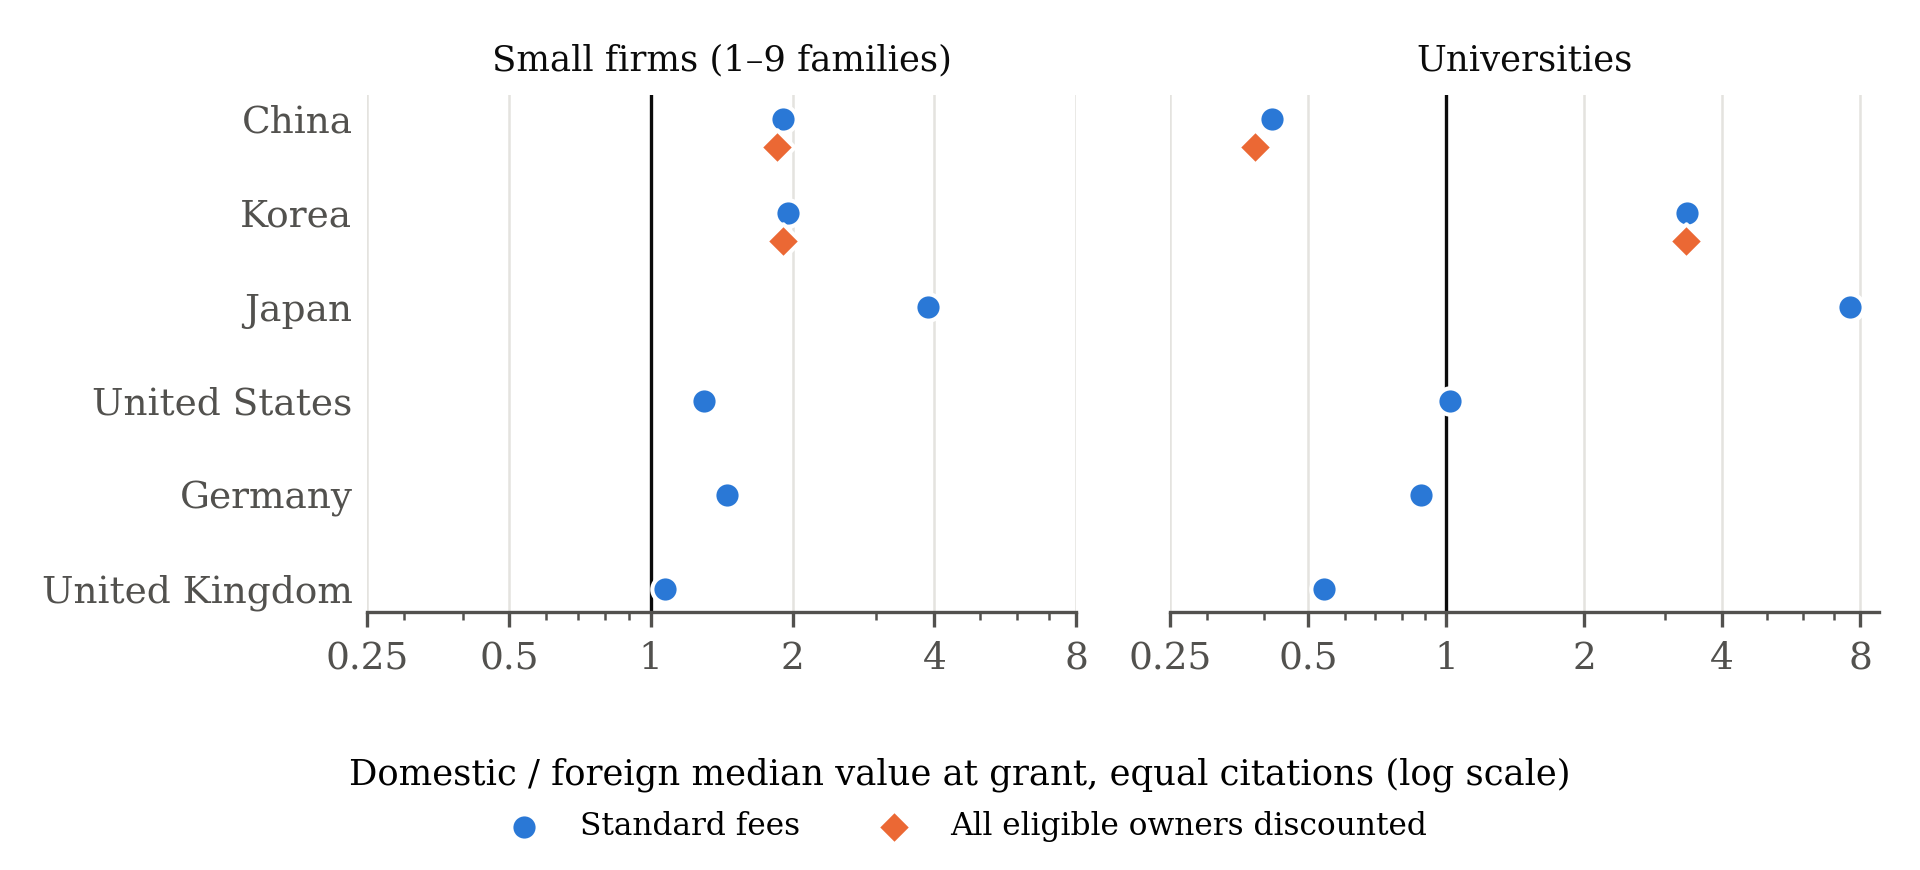
\includegraphics[width=0.9\textwidth]{figures/fig4_value_ratios.png}
\caption{Value of domestic relative to foreign owners' patents in the same office}\label{fig:values}
\figurenotes{Ratio of domestic to foreign owners' median patent value at grant, with citations at the office median,
from the deterministic renewal model ($d=0.85$, discount factor 0.9, fees in 2024 PPP dollars). Filled circles:
standard fees. Diamonds: every eligible domestic owner (firms with 1--99 families and universities) pays the
discounted fee in China and Korea, a lower bound for domestic values. Open circles: Russia, where the model is not
identified (see text). Log scale.}
\end{figure}

\paragraph{Fee discounts do not explain it.} China and Korea cut renewal fees for domestic small firms and
universities, and the models above assume standard fees. Lower fees mean the same renewal behaviour implies lower
values, so I re-estimate both models assuming that every eligible owner took the discount: in China, 30\% of the fee
in the first three fee-years after grant until 2016 and 15\% for up to ten years from 2018; in Korea, 70\% of the fee
in years 4--6 from 2014 and half from 2018. Values fall by a few percent (Figure~\ref{fig:values}): the ratio for
small firms is 1.85 in China and 1.91 in Korea in the deterministic model, and 1.61 and 1.51 in the learning model.
The discounts apply when fees are low, about \$250--350 a year in China, against values in the tens of thousands.

\paragraph{Patent-level values.} Group means could hide the patents that matter. I therefore value each patent from
its own renewal history: the learning model is re-estimated with a single prior for all owners, in which only
citations enter, and each patent's value is the posterior median over simulated return paths, weighting each path by
the probability of the patent's observed lapse or survival. Owner type plays no role in a patent's value. Regressing
log value on domestic owner by size, with fee-path $\times$ citation-band and office $\times$ field effects,
Table~\ref{tab:patentvalues} shows that small domestic firms' patents are worth about 20\% more than small foreign
firms' in China and 30\% more in Korea, as in the United States and Germany, and the same in the Czech Republic and
France. In Taiwan they are worth 18\% less. Chinese universities' patents are worth 58\% less than foreign
universities' ($1-e^{-0.87}$).

\begin{table}[t]
\centering
\begin{threeparttable}
\caption{Patent-level values, domestic minus foreign owners (log points)}\label{tab:patentvalues}
\small
% Source: em-patent-value output/patent_value_gaps.csv, patent_value_gaps_RU_TW_CZ_FR.csv (21_patent_values.py)
\begin{tabular}{lcc@{\hspace{2.5em}}lcc}
\toprule
Office & Small firms & Universities & Office & Small firms & Universities \\
\midrule
China          & 0.20 (0.03)    & $-0.87$ (0.07) & United States  & 0.22 (0.02)    & 0.13 (0.20) \\
Korea          & 0.26 (0.06)    & 0.44 (0.19)    & Japan          & 1.11 (0.07)    & 1.94 (0.55) \\
Russia\tnote{a} & $-0.45$ (0.64) & --            & Germany        & 0.21 (0.06)    & $-0.19$ (0.33) \\
Taiwan         & $-0.20$ (0.09) & 1.77 (0.32)    & United Kingdom & $-0.05$ (0.06) & $-0.59$ (0.15) \\
Czech Republic & 0.07 (0.21)    & $-0.20$ (0.57) & France         & 0.00 (0.08)    & $-0.48$ (0.27) \\
\bottomrule
\end{tabular}
\begin{tablenotes}\footnotesize
\item \emph{Notes:} Posterior median value at grant of each patent from the learning model with a common prior
($d=0.85$; 2024 PPP dollars), regressed on domestic owner $\times$ owner group with fee-path $\times$ citation-band and
office $\times$ field effects; standard errors clustered by owner. 1.37 million patents. Japanese university estimates
are unstable across specifications.
\item[a] Not identified (see text); no foreign university patents in the Russian estimation sample.
\end{tablenotes}
\end{threeparttable}
\end{table}

\paragraph{Levels are rough; ratios are not.} A typical small domestic firm's patent is worth roughly
\$5{,}000--60{,}000 at grant in the deterministic model and several times more in the learning model, in which early
lapses reflect learning rather than low initial value. Values in different offices also cover protection in
different markets. The ratios, on which the argument rests, are stable across models, decay rates and fee
assumptions, except in Russia. Because a patent's value on a given fee path rises with how long it is kept, the
patent-level values restate the survival results in money rather than adding an independent test.

\section{Conclusion}\label{sec:conclusion}

The apparent emerging-market gap in patent survival is mostly a matter of when the renewal clock starts and of what
gets patented. Counted from grant and at equal observable quality, Chinese and Korean firms keep and value their
patents much as firms in the United States, Japan, Germany and the United Kingdom do. Credit shocks and fee cuts
barely move their renewal decisions, and they do not drop home patents of inventions they still protect abroad.
For firms, the binding constraint is the invention, not the inventor.

Owner capacity matters at the margin: small emerging-market firms' patents survive much longer after a sale,
especially to another company. Policies that deepen markets for technology, such as registries, licensing
intermediaries and secure transfer of title, may therefore add value. Short-run credit or fee relief is unlikely to
change which patents are kept. The clear weak spot is university patenting in China, where patents are dropped
sooner and are worth well under half as much as comparable foreign ones, consistent with patenting driven by
evaluation and subsidy targets rather than use.

Three limitations stand out. ``Emerging markets'' here means mainly China and Korea; Brazil is too thin, and other
large emerging economies do not report lapses in PATSTAT. Citations do not capture every dimension of quality.
And the structural values assume standard fees, while small domestic owners in China and Korea can claim fee
reductions; bounding that effect is left to a revision. % TODO: fee-discount bounds; additional offices.


\bibliographystyle{plainnat}
\bibliography{references}

\appendix
\section{Additional results}\label{sec:appendix}

\begin{table}[ht]
\centering
\begin{threeparttable}
\caption{Domestic minus foreign owners, alive 8 years after grant, by office (pp)}\label{tab:byoffice}
\small
% Source: em-patent-value notes section 9 (16c_survival_from_grant.py)
\begin{tabular}{lcccc}
\toprule
Office & Individuals & Firms, 1--9 & Firms, 100--999 & Firms, 1{,}000+ \\
\midrule
China   & $-$19.8 & 7.4    & 19.4   & 8.7 \\
Korea   & 0.3     & 10.6   & 18.7   & 9.0 \\
US      & $-$3.6  & $-$2.2 & 6.2    & 4.3 \\
Japan   & 8.4     & 21.4   & 25.4   & 14.0 \\
Germany & $-$6.3  & 3.4    & 7.5    & 3.7 \\
UK      & $-$13.5 & $-$3.7 & $-$1.3 & 25.2 \\
\bottomrule
\end{tabular}
\begin{tablenotes}\footnotesize
\item Notes: Within-office comparisons with citation and field controls. Individuals are shown for reference; they are
excluded from the main analysis.
\end{tablenotes}
\end{threeparttable}
\end{table}

\begin{table}[ht]
\centering
\begin{threeparttable}
\caption{Learning model: rate of decline and fit}\label{tab:learning}
\small
% Source: em-patent-value notes section 14 (20_learning_model.py)
\begin{tabular}{lcccccc}
\toprule
 & China & Korea & Japan & US & Germany & UK \\
\midrule
Free estimate of $d$ & 0.47\tnote{a} & 0.67\tnote{a} & 0.73\tnote{a} & 0.47\tnote{a} & 0.851 & 0.840 \\
$\sigma_0$ at $d = 0.85$ & 1.12 & 1.34 & 3.07 & 2.63 & 1.52 & 1.81 \\
Shock $s$ & 0.99 & 0.62 & 1.05 & 0.34 & 1.02 & 1.05 \\
Learning $\varphi$ & 0.95 & 0.99 & 0.98 & 0.99 & 0.86 & 0.85 \\
Mean absolute fit error (pp) & 2.9 & 3.7 & 2.7 & 1.6 & 2.4 & 2.1 \\
\bottomrule
\end{tabular}
\begin{tablenotes}\footnotesize
\item Notes: Fit error: predicted minus observed share alive at 4, 8 and 12 years after grant, by owner group.
\item[a] Not identified: the estimate comes with an implausibly wide spread of initial values and values in the
millions.
\end{tablenotes}
\end{threeparttable}
\end{table}


\end{document}
